%%%%%%%%%%%%%%%%%%%%%%%%%%%%%%%%%%%%%%%%%%%%%%%%%%%%%%%%%%%%%%%%%%%%%%%
%% February 10, 2018
%%
%%%%%%%%%%%%%%%%%%%%%%%%%%%%%%%%%%%%%%%%%%%%%%%%%%%%%%%%%%%%%%%%%%%%%%%
\documentclass{article}[12pt,preprint]
\textwidth 17cm
\textheight 26cm
\hoffset -2.5cm
\voffset -4.5cm

\usepackage{xcolor,color}
\usepackage{graphicx}
\usepackage{amsmath,amssymb}
\usepackage[colorlinks=true,linkcolor=blue]{hyperref}

\begin{document}

\title{\mbox{\large
	\underline{Proposal for Project at Center for Nuclear Femtography}}
\vspace{0.6cm}
\\ \emph{Navigating the scientific literature with AI}
\vspace{0.2cm}
}

\author{
  N.~Sato$^{1,2}$,
  A. Trewartha$^{3}$ 
	W.~Melnitchouk$^2$,
	\vspace{0.3cm}
\\
$^1${\it Old Dominion University},
$^2${\it Jefferson Lab},
$^3${\it Berkeley Lab }}

\vspace{-6ex}

%\date{\today}
\date{}

\maketitle

\noindent \color{black}

%%%%%%%%%%%%%%%%%%%%%%%%%%%%%%%%%%%%%%%%%%%%%%%%%%%%%%%%%%%%%%%%%%%%%%%%%
\section{Project outline}

The goal of the project is to build a comprehensive scientific
{\it literature explorer} using artificial intelligence (AI),
tailored for nuclear and high energy particle physics.
%
Currently, a large fraction of researchers' time is invested in 
searching the scientific literature.  The proposed AI will allow
for efficient and automatic extraction of scientific results,
dramatically boosting research productivity.
%
It will be equipped with intelligent decision making tools and 
strategies that will aid the user in exploring and creating insights 
from thousands of scientific papers, highlighting relevant manuscripts 
individualized for each query.
%
{\color{red}[Maybe mention Watson, materials project, etc??] refs }

%
For this we plan to:

\begin{itemize}

\item
{\it Design natural language processing} (NLP) {\it algorithms} that
can efficiently interpret the user's queries, as well as automatically
extract relevant information contained in papers in the form of graphs,
tables, equations or scientific statements.  Each of these are
independent skills that can be developed separately.

\item
{\it Construct a database of scientific results} for the AI explorer
to store the collected and processed information from the literature.
The result will be a \emph{universal data hub} (UDH) that can be
regularly updated with the latest scientific results.

\item 
Since the information contained in the literature will be transformed
from the into the UDH internal representation, it avoids the need to
achieve community consensus on standard data storage formats, as well as
allowing efficient integration of historic results.
We will consequently {\it develop apps that can transform and transfer
the information} to the user's desired formats.

\end{itemize}

%%%%%%%%%%%%%%%%%%%%%%%%%%%%%%%%%%%%%%%%%%%%%%%%%%%%%%%%%%%%%%%%%%%%%%%%%
\section{Deliverables by July 1, 2019}

While the completion of the project is a long-term goal, we plan in the
short term to develop a prototype for the AI explorer's graph extraction capability. 

{\color{red}

- what do we mean by graph extraction app.

- Also state that extraction is different from understanding. 
  What would be "understanding"?  

- How we will achieve that? 
 
  + existing software refs 
  + what are the samples to train the AI
  + what computing capabilities are needed
  + what kind of workforce we need

- How/where we are planning to make it available to public. AWS?, JLab
  servers? 

}

%%%%%%%%%%%%%%%%%%%%%%%%%%%%%%%%%%%%%%%%%%%%%%%%%%%%%%%%%%%%%%%%%%%%%%%%%
\section{Budget}

The project requires an interdisciplinary collaboration with a
machine learning (ML) group from an academic institution that
has expertise in natural language processing algorithms, data
visualization, and data management.  To achieve this, we request
the following:

\begin{itemize}

\item
Funding to purchase dedicated machines equipped with CUDA-enabled
GPUs for development and training of the AI as well as the
server to host the interactive web space.  The machines will be
stationed at Jefferson Lab and the collaborators will have access
to the machines remotely.

\item
Funding for travel to Jefferson Lab for the collaboration personnel.

{\color{red} ...[specify how much travel, length of visits,
\$ amounts?]...}

\end{itemize}

{\color{red} ...[this looks very similar to the other proposal]...}



%------------------------------------------------------------------------
\begin{figure}[!h]
\centering
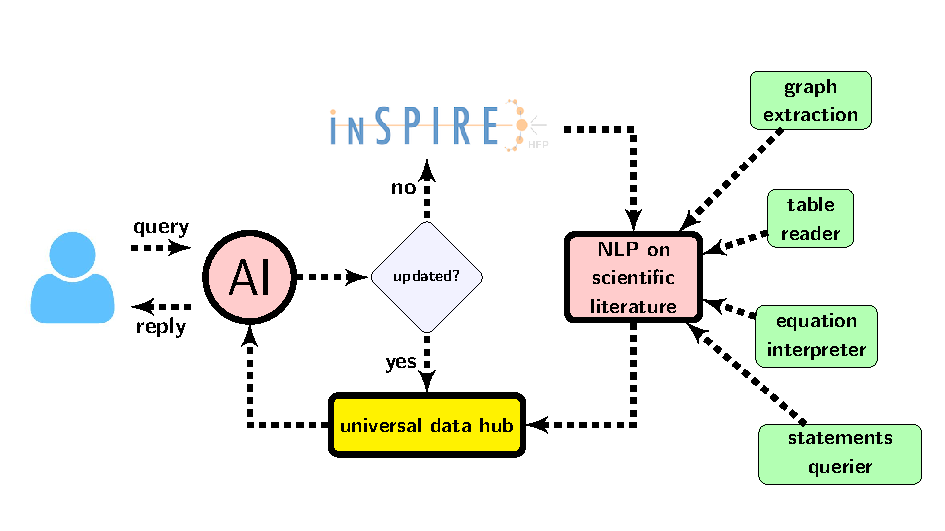
\includegraphics[width=1\textwidth, angle=0]{gallery/ai}  
\caption{Schematic view of the proposal.}
\label{f.1}
\end{figure}

%%%%%%%%%%%%%%%%%%%%%%%%%%%%%%%%%%%%%%%%%%%%%%%%%%%%%%%%%%%%%%%%%%%%%%%%%
\begin{thebibliography}{99}

\bibitem{JAM}
Jefferson Lab Angular Momentum (JAM) Collaboration,
{\tt https://www.jlab.org/jam}.

\bibitem{PARTONS}
B.~Berthou {\it et al.},
Eur. Phys. J. C {\bf 78}, 478 (2018).

\end{thebibliography}

\end{document}
